\chapter{Architecture}%
\label{chap:architecture}
The architecture for the application is composed by the user's device and a server, hosted on Google Firebase.
\begin{figure}[htpb]
    \centering
    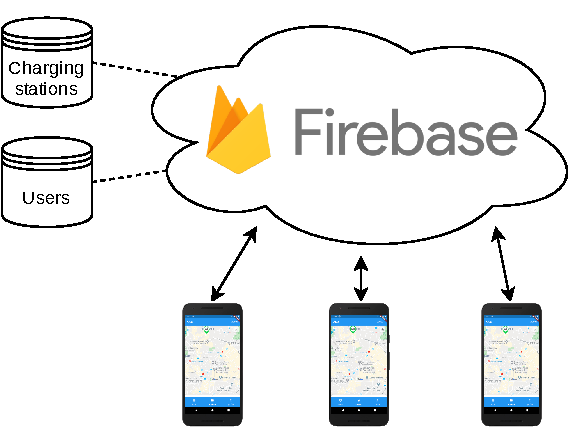
\includegraphics[width=0.9\linewidth]{Pics/architecture.pdf}
    \caption{Basic architecture of the application.}%
    \label{fig:Pics/architecture}
\end{figure}
In this diagram the two main components are shown:
\begin{itemize}
    \item Mobile app: the user can interact on their device in order to retrieve the recharging stations and their data, along with the functionalities cited in\ref{chap:ideaAndRequirements}.
    \item Firebase: Google Firebase offers a simple way to blabla
\end{itemize}

\section{Use case diagrams}%
\label{sec:use_case_diagrams}
\begin{figure}[H]
    \subfloat[]{
	\begin{tabular}{|l|p{0.6\linewidth}|}
	    \hline
	    Name & Sign up \\
	    \hline
	    Actor & User \\
	    \hline
	    Entry conditions & User has AlGa app installed on their smartphone \\
	    \hline
	    Events flow & \begin{enumerate}
			    \item Click the ``Sign Up'' button
			    \item Fill the form providing the requested information
			    \item Click the ``Confirm button''
			    \item User is now enrolled to AlGa.
			  \end{enumerate}\\
	    \hline
	    Exit conditions & The app shows the main screen to the user.\\
	    \hline
	    Exceptions & \begin{enumerate}
			    \item The e-mail is already taken.
			    \item The format for e-mail or password is wrong.
			    \item All the exceptions are handled by notifiying the user and taking him back to the main screen.
			\end{enumerate}\\
	    \hline		
	\end{tabular}
    }\quad
\end{figure}
\begin{figure}[H]
    \subfloat[]{
	\begin{tabular}{|l|p{0.6\linewidth}|}
	    \hline
	    Name & Login \\
	    \hline
	    Actor & User \\
	    \hline
	    Exit conditions & The app shows the main screen to the user.\\
	    \hline
	    Events flow & \begin{enumerate}
			    \item The user opens the app
			    \item The user fills the ``E-mail'' and ``Password'' fields
			    \item The user clicks on the ``Login'' button
			  \end{enumerate}\\
	    \hline
	    sxit conditions & The app starts to show the collected data to the user \\
	    \hline
	    Exceptions & \begin{enumerate}
			    \item The e-mail is not associated with a registered user
			    \item The password is not correct for the given e-mail
			    \item All the exceptions are handled by notifiying the user and taking him back to the main screen.
			 \end{enumerate}\\
	    \hline		
	\end{tabular}
    }\quad
\end{figure} 
